\chapter{Methods}
In this chapter we review the basic implementation details of our distributed
video processing cloud architecture. First we cover the overall distributed
architecture on the cloud.  We delve into details of how all the compute nodes
communicate with the primary node and how this can be done at any scale. Another
step we take in this thesis,  is to cover the development process and release
process utilized for this open source package. The details of continuous
integration and test driven development are  important driving factors in
developing reliable, scalable, and useable code.  Then we cover how we use
Lucas-Kanade and Farneback optical flow algorithms to reduce the feature space
to only six 25 bin feature vectors. Finally, with the reduced feature space, we
outline how to classify the videos using several well known machine learning
algorithms such as K-nearest neighbors and support vector machines (SVM).

\section{\label{section:distributed_processing}Scalable Architecture}
A core principal for a well designed, horizontally scalable application, is
to design it such that it does not contain state \cite{awsbestpractices}.
When state is required, the software complexity increases substantially and
makes it difficult to distribute the system over a scalable amount of nodes.
However, if the software was designed such that each service can operate and
stand on its own, it is the perfect embarrassingly parallel computing task to
tackle. For this thesis we focus on ensuring that our feature extractor,
as described in Section \ref{section:feature_extraction}, is completely stateless.
This is a design feature that has allowed us the flexibility to scale our
system over as many nodes as are available on the AWS cloud. A stateless architecture
greatly increases the chances of any program to be turned into a micro service
on the cloud. As a result, more and more parts of any application can  be horizontally scaled
across any number of compute nodes. So unless access to stateful services are
necessary, such as database accesses, it is almost always best to design
software stateless to create scalable services. This also has the added advantage


\subsection{\label{subsection:architecture_overview}Architecture Overview}
Our system builds upon AWS to create an easy-to-maintain and easy-to-scale
video processing system. We use S3 storage to put small video clips that
have been extracted from our AOLME dataset. These clips are made available to
to all processing nodes. The processing nodes communicate with the master
node using Amazon's simple queue service (SQS). Figure \ref{fig:dataflow} illustrates
the basic distributed system design and the psuedo-code for the entire system
is shown in Figure \ref{alg:pseudo_master_node} and Figure \ref{alg:pseudo_compute_node}.

\begin{figure}[h]
  \centering
  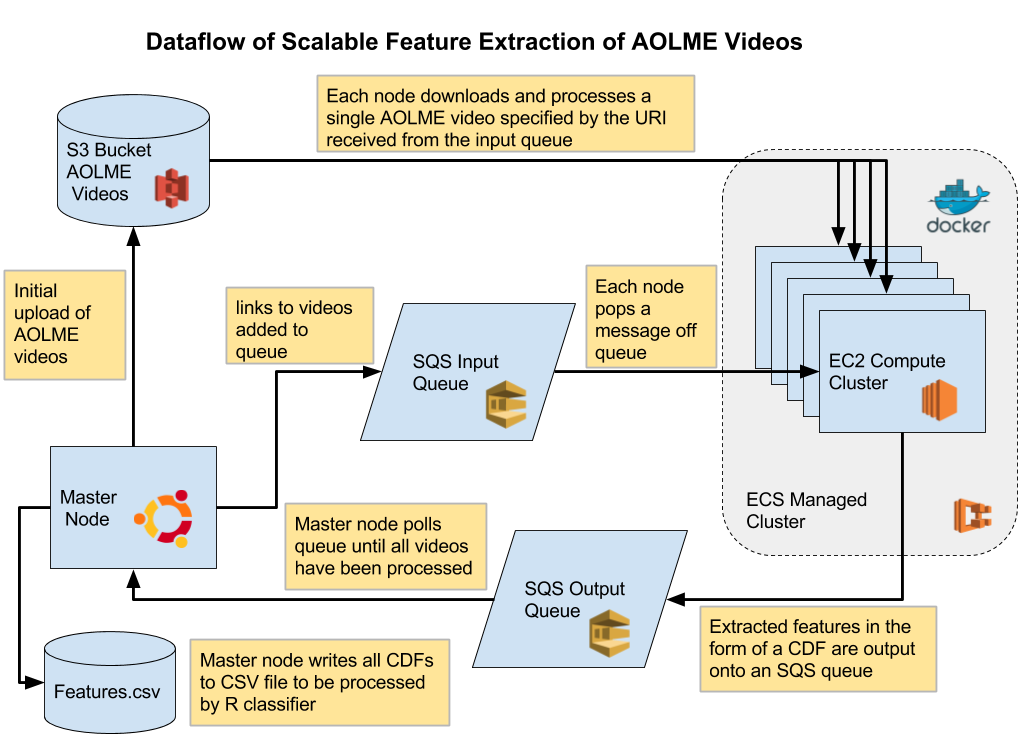
\includegraphics[width=\textwidth]{figures/extract_features_dataflow}
  \caption{Dataflow of the distributed video system using AWS components}
  \label{fig:dataflow}
\end{figure}

\begin{figure}[h]
\begin{algorithmic}[1]

  \For{each \textit{video} in pre-segmented videos}
    \State $\texttt{UploadToS3(}\textit{video}\texttt{)}$
  \EndFor
  \State $\texttt{AddVideosToSqsQueue(}\textit{video\_list.txt}\texttt{)}$

  \While{videos in \textit{video\_list.txt} are still in processing}
    \State $\texttt{Sleep(1)}$
  \EndWhile

  \State $\textit{output.txt} = \texttt{WriteCdfsToFile(PopAllCdfsFromQueue(}\textit{output\_queue\_name} \texttt{))}$

  \State $\textit{dataframe} = \texttt{ReadCsv(} \textit{output.txt} \texttt{)}$

  \For{\textit{sample\_index} in 1 to len(\textit{dataframe})} \Comment{Leave-one out algorithm for training and testing}
    \State $\textit{train\_data} = \textit{dataframe[-sample\_index]}$
    \State $\textit{test\_data} = \textit{dataframe[sample\_index]}$
    \State $\textit{knn\_result} = \texttt{knn(}\textit{train\_data, test\_data, k=3} \texttt{)}$
    \State $\textit{svm\_model} = \texttt{svm(}\textit{train\_data, kernel=linear, cost = 0.001...10000} \textit{)}$
    \State $\textit{svm\_result} = \texttt{predict(} \textit{svm\_model, test\_data} \texttt{)}$
  \EndFor
  \State $\texttt{WriteExperimentResults(} \textit{knn\_result, svm\_result} \texttt{)}$

\end{algorithmic}

\caption{Pseudocode for proposed method in the master node. In the above pseudo-code, indentation
indicates the beginning and end of a block of code, in other words when the
indentation ends in a for loop, it means that is the end of the for loop. Additionally,
all function names represent the same function names that were created in the actual
code.}
\label{alg:pseudo_master_node}

\end{figure}

\FloatBarrier

\begin{figure}[h]
\begin{algorithmic}[1]
  \State $\textit{video\_uri} = \texttt{PopVideoFromQueue()}$
  \State $\textit{segmented\_video} = \texttt{DownloadS3Video(}\textit{video\_uri}\texttt{)}$
  \State $\textit{previous\_frame} = nullptr$

  \For{each \textit{frame} in \textit{segmented\_video}} \Comment{Block  extracts features from video frames}
    \State $\textit{current\_frame} = \textit{frame}$
    \If {\textit{previous\_frame} == nullptr}
      \State $continue$
    \EndIf
    \State $\textit{optical\_flow} = \texttt{CalculateOpticalFlow(}\textit{current\_frame, previous\_frame} \texttt{)}$
    \State $\textit{mag} = \textit{optical\_flow}.\texttt{GetMagnitude()}$
    \State $\textit{max\_mag} = \texttt{Max(} \textit{mag} \texttt{)}$
    \State $\textit{magnitude} = \textit{mag} > \textit{max\_mag} \times 0.25$
    \State $\textit{orientation\_vectors} = \textit{optical\_flow}.\texttt{GetOrientations()}$
    \State $\textit{blobs} = \texttt{GetBlobs(} \textit{magnitude}\texttt{)}$
    \For{each \textit{blob} in \textit{blobs}}
      \State $\textit{centroid\_x, centroid\_y} = \texttt{GetCentroids(} \textit{blob} \texttt{)}$
      \State $\textit{blob\_orientations} = \texttt{GetBlobOrientations(} \textit{blob} \texttt{)}$
      \State $\textit{background\_mag} = \texttt{GetMotionAround(} \textit{mag, blob} \texttt{)}$
    \EndFor
    \State $\textit{num\_bins} = 25$

    \State $\textit{pdfs} = \texttt{GetPdfs(} \textit{magnitude, orientation\_vectors} $
    \Statex $\textit{centroid\_x, centroid\_y, blob\_orientations, background\_mag, 25} \texttt{)}$
  \EndFor
  \State $\textit{cdf\_features} = \texttt{Normalize(}\textit{pdfs}\texttt{)}$
  \State $\texttt{PushToSqsQueue(}\textit{cdf\_features}, \textit{output\_queue\_name} \texttt{)}$

\end{algorithmic}

\caption{Pseudocode for proposed method. In the above pseudo-code, indentation
indicates the beginning and end of a block of code, in other words when the
indentation ends in a for loop, it means that is the end of the for loop. Additionally,
all function names represent the same function names that were created in the actual
code.}
\label{alg:pseudo_compute_node}

\end{figure}

From Figure \ref{fig:dataflow} we see that the first step is to upload
the videos to S3. We keep the videos very small, because as we show in our experiments
section, it takes quite a long time to process large videos therefore there is a
significant benefit to keeping the video chunks relatively small so that many
machines could potentially work on the feature extraction process. The next step
is to place a message on the SQS queue specifying which video to process and
what its classification is. For the purposes of this thesis, we manually place
messages on the queue so that we can control the flow of messages. In
a production system though, we would have the S3 bucket notify the SQS queue that
a new video was uploaded and ready for processing. The third step is the processing
step. In our setup, we create 20 EC2 instances running our feature extractor application.
Each one of these instances polls the SQS queue waiting for a message to arrive.
As soon as one does, it downloads the appropriate video from the S3 bucket,
processes the video, and then places the results on another SQS queue. At this
point, the master node is polling the results queue and collecting the results
into a csv file. Finally, the csv file can be used to train the SVM in the R
code.

\subsection{\label{subsection:master_node}Master Node Configuration}
The master node in our system is responsible for sending out jobs to process and
then coalescing the results from the calculations performed by the slave nodes.
All of these processes are done using the boto3 \cite{boto3} Python  software
development kit (SDK). The core implementation of AWS uses a  representational
state transfer like (RESTful) interface to communicate to all the services that
Amazon offers in a programatic  way, but they also offer several easy-to-use
object oriented libraries written  in several languages to make programming easier
for the end user. The master node
need not be any specific operating system as long as the Python language
can be interpreted on it. In this thesis, we use Ubuntu 14.04 to run our master
node logic, but it could just as well be OS x or any other flavor of linux.

The master node performs several basic tasks. The first of which is to put
messages on the SQS queue.  This is orchestrated by reading
a csv file that consists of an S3 link to a video segment, the classification of
the segment, the SQS queue to which to output the features and finally the
optical flow method to use. An example of the file is shown in Table
 \ref{tab:message_queue}.

\begin{table}[h]
  \begin{tabular}{ | l | l | l | p{2cm} |}
  \hline
  \textbf{path} & \textbf{classification} & \textbf{sqs\_queue} & \textbf{algorithm}\\ \hline
  aolme/data/typing/seg\_1.mp4 & 1 & feature\_queue & farneback \\ \hline
  aolme/data/notyping/seg\_1.mp4 & 2 & feature\_queue & farneback \\
  \hline
  \end{tabular}
  \caption{Example of data file that is used by the master node to place messages on
  the SQS queue. }
  \label{tab:message_queue}
\end{table}

\FloatBarrier

From the example data shown in Table \ref{tab:message_queue}, we can see that
the nodes have the ability to switch the algorithm as well as associate a
classification from the video. Having the ability to switch method types allows
us to easily benchmark using Lucas-Kanade optical flow versus Farneback.
We also put the output queue in the message so that the slave nodes know to which
queue to place the results of their calculations. This information is also necessary
for the master to know which queue to wait on to collect all the results. Additionally,
if we need more information to be passed to the slave nodes so that they can
effectively do their job, we can easily put that information in the queue with
the message trivially.

Once the master node has sent all the messages to the queue, it then polls
on the queue it placed the messages on to verify that all the messages have been
remove by the slave nodes. This is an important step to validate that the
slave nodes are indeed popping messages off the SQS queue and processing
the videos that are associated with each message. Once this has been validated,
the master node begins to poll on the designated output queue for the results output
from each of the slave nodes. Once all the results have been collected, the master
node places each of the vectors into a comma separated features file.
The pseudo code for the operations performed by the master are shown in Figure
\ref{alg:master_node}.

\begin{figure}[h]
\begin{algorithmic}[1]
  \State $videos\_to\_process \gets \texttt{ReadInputData(input.csv)}$
  \For{\texttt{i = 0; i < len(videos\_to\_process); ++i}}
    \State $sqs\_message \gets \texttt{CreateMessage(videos\_to\_process[i])}$
    \State $output\_queue\_uri \gets videos\_to\_process[i].output\_queue\_uri$
    \State$\texttt{SendSqsMessage(}sqs\_message, sqs\_uri \texttt{)}$
  \EndFor

  \While{$\texttt{MessagesRemainingInQueue(}sqs\_uri \texttt{)} \neq 0$} \Comment{Poll queue every second}
    \State $\texttt{Sleep(1)}$
  \EndWhile

  \While{$\texttt{MessagesRemainingInQueue(}output\_queue\_uri\texttt{)} \neq 0$}
    \State $feature\_vectors \gets \texttt{ReceiveSqsMessage(output\_queue\_uri\texttt{)}}$
    \State $\texttt{Sleep(1)}$
  \EndWhile

  \State \texttt{WriteFeaturesToDisk(} $feature\_vectors$ \texttt{)}

\end{algorithmic}
\caption{Pseudo code for collecting the features in the master node}
\label{alg:master_node}
\end{figure}

As we have shown in this section, very little needs to be configured on the master
node other than the ability to run Python and the AWS python utilities. This
makes running our software from almost any type of machine very easy with just a
few setup steps. The master node plays an important role in sending and receiving
the data that the user wishes to process and is an enabling part of our system.
That is to say, it really doesn't matter what software we are running on our
slave nodes, as long as the slave nodes fulfill the contract that we have
defined in our messaging format. This means that we don't necessarily have to
run our C++ extract features program on the slave nodes, but we could be running
any flavor of algorithm we wish with no configuration changes on the master node.
Not only is this setup scalable, but it's highly flexible because of this idea.

\subsection{\label{subsection:slave_node}Slave Node Configuration }
The next very important piece to our innovative architecture is the algorithm
that is run on all the slave nodes. This algorithm simply polls on a single
queue, then once a messages is received, it downloads the small S3 video
segment, processes it using our feature extraction technique, puts the results
on a queue that it has discovered on the incoming message, deletes the video
locally and then begins polling on the queue again. Figure \ref{alg:slave_node}
illustrates this idea clearly.

\begin{figure}[h]

\begin{algorithmic}[1]

  \While{$True$}
    \State $sqs\_message \gets \texttt{ReceiveMessages(} queue\_name \texttt{)}$ \Comment{Blocking call}
    \State $video\_path \gets \texttt{DownloadS3Video(} sqs\_message.video\_path \texttt{)}$
    \State $features\_cdf \gets \texttt{ExtractFeatures(} video\_path \texttt{)}$ \Comment{Call C++ Code}
    \State $\texttt{SendS3Message(} sqs\_message.output\_queue, features\_cdf \texttt{)}$
    \State $\texttt{DeleteSqsMessage(} sqs\_message \texttt{)}$ \Comment{Remove message from queue}
    \State $\texttt{Sleep(1)}$
  \EndWhile
\end{algorithmic}
\caption{Slave Node Implementation Pseudo-Code}
\label{alg:slave_node}
\end{figure}

We can see that the slave node logic is, like the master node, very simple. We
simply wait for messages to come in from one queue, process the video, and then
output the features onto another queue. However, there is a piece missing from
Figure \ref{alg:slave_node} that makes the slave nodes a truly innovative
part of our overall architecture and that is the orchestration and deployment
of our highly refined C++ code.

One of the big hurdles in launching applications that run on a cluster is that
all the nodes on the cluster must be running the same libraries, operating
system,  and versions of the software so that all the answers are returned from
the slaves are repeatable and reliable. In traditional systems, this action was
typically performed by system admin and as a result, you had to rely on third
party packages and libraries that were deployed with the cluster. So if the
software under development needed some updates to a package or some bug fixes,
you were out of luck. You had  to work around those bug fixes and/or write the
updates by hand to get similar  functionality. This is not so with our system.
Using ECS, EC2 and Docker \cite{Merkel:2014:DLL:2600239.2600241}, we  have
developed a system that allows any flavor of linux to be deployed with any
version of software that is required to run on the slave nodes seamlessly. For
example, we developed our C++ code using OpenCV 3.0 and g++4.8 all on Ubuntu
14.04 and built a Docker container that packaged all that software together.
We were then able to deploy our software to an Amazon machine image (AMI) running
an Amazon flavor of Linux that was built for running docker and for communicating
to an ECS cluster. We did all that without configuring a single Linux instance
by hand. And should we choose to roll back to an earlier version of OpenCV or
upgrade our compiler to the latest standard, we could do so by changing the
configuration of our Docker container and our development environment. This
method in no way hinders either vertical or horizontal scalability. With Docker,
we can still pass flags that allow the container to take over the host's GPUs
so that any code written specifically for the GPUs can still be run in a container.


\section{\label{section:auto_deployment}Automatic Deployment of Software and
the Development Process}
An aspect of this thesis that separates us from many of the techniques proposed
in the background section, is the way we have developed our system to be readily
repeatable, easy to use and flexible to allow to future improvements. This is
especially important to UNM's image and video processing and communication lab
ivPCL lab so that future graduate students can leverage the work done in this
thesis to get a head start on future developments of the proposed feature
extraction algorithm. In this section we cover several topics that demonstrate
that we have done more than just provide an innovative solution to classifying
activities in video, but have also created a system after which other projects
can model themselves. Specifically, we cover how the proposed architecture's
underlying C++ code is developed and how it is automatically and seamlessly
deployed to AWS all the while maintaining a vertically and horizontally scalable
architecture.

\subsection{\label{subsection:opencv_tapi}Vertical Scalability}
Since the ivPCL is strongly geared towards vertically scalable solutions using
FPGAs and GPUs, it is fitting that we should also make the goal of this thesis
to leverage those technologies. To do so, we have developed our software to take
advantage of OpenCV's transparent API known as TAPI. The transparent API is an
enabling technology to be able to seamlessly switch between GPU, CPU and or any
hardware technologies without the software programmer having to select one at
compile time or at run time explicitly. TAPI uses Open Computing Language
(OpenCL) has its underlying technology to achieve significant improvements over
its base algorithm suite. This fundamental technology allows the programmer to
write software for a variety of hardware implementations without being burdened
with implementing the algorithms by hand. For example, the Farneback optical
flow algorithm that is already provided in the OpenCV library can be run easily
on either the GPU or the CPU with almost no extra programming on the programmers
part. This is also a powerful idea for users who want to distribute software to
wide community, but have hardware accelerations that can be added to speed the
software up when the hardware is available on the system. So if the programmer
has attached an accelerated algorithm for computing the discrete radon transform
as demonstrated in \cite{Cesar2014a}, it is completely possible to plug that
implementation into OpenCL and in turn, program the abstraction layer into the
OpenCV library. This also means that the horizontally scalable aspect of this
thesis still holds so that we can distribute the same algorithm to nodes with
less capable hardware. Although it is optimal to have a cluster of machines with
FPGAs hanging from the PCI express bus, implementing the software in OpenCL
gives users the option to run the code on almost any compute device. This means
that the code can run on machines in AWS or in a local cluster. Furthermore,
machines that have the necessary hardware and are accessible in the lab can
perform some of the heavy lifting before farming out the rest of the data to the
slave nodes on the AWS cloud. So even though the system is designed with
horizontal scalability in mind, the option of going vertically scalable for
certain computations has been in no way hindered.

\subsection{\label{subsection:cont_integration}Continuous Integration}
Its all too often that software is written and completely forgotten about
because the build process is too complicated and burdensome on the users of the
interface.  A goal of this thesis is to maximize reusability and maintainability. We
accomplish this using a popular software technique called continuous
integration \cite{duvall2007continuous}. Continuous integration is the idea that
software should be constantly giving developers feedback about the state of
their software to ensure robustness and to have an obvious tool for developers
to use document the build process of the software. This is an especially
important tool for teams of developers so that failures of new commits
can easily be observed quickly and effectively. This has the advantage of addressing
errors early on in the software development phase so that errors are addressed
immediately.

For this thesis, we chose to use an online tool called Travis-CI for our
continuous integration. Travis easily hooks into our Github repository and
automates the build process of our extract features program. The build of our
C++ program consists of compiling and linking against all third party libraries,
running all of our google test unit tests, and then deploying the Docker image
to AWS to be used for deployment on the ECS cluster. This tool significantly
unburdens the developer from having to do these steps manually. Continuous
integration also ensures that the unit tests that have been developed for the
software work on the deployed environment specifically in the docker image. In
other words, we develop the software locally on any flavor of linux,  but there
is a chance that any new changes that we have made to the software do not work
in the deployed system. Travis-CI acts as an automated alert that something might
not be right in the software.

The fact that the continuous integration also pushes our Docker image up to  our
ECS cluster is also huge advantage. This process  ensures that  our Cluster is
always running the latest compiled and unit tested version.  So not only have we
made deployment of our software easy using a Docker  container to package it up,
we've also automated the entire deployment process of our software simply by
pushing our code to our Github repo.

Making the deployment and build of our software automated has guaranteed us
that we will have repeatability in our code and that we have the latest
functioning version running on our compute cluster. Furthermore, if mistakes are
made at the local development level and they are not caught until the developer
has pushed their changes to a Git repo, the automated build system will trigger
a failure and not deploy the system. A key contribution with using the automated
build system is that anyone from anywhere will be able to repeat the experiments
that we have performed in this paper with very little software configuration. We
have essentially frozen the code in a working state. Even if AWS goes away, the
core Docker image is available to be run on any *nix type machine with Docker installed.
So if future users decide that they want to use our extract features algorithm,
it is ready to run. Figure \ref{fig:continuous_integration} illustrates the
general flow of the continuous integration.

\begin{figure}[h]

  \centering
  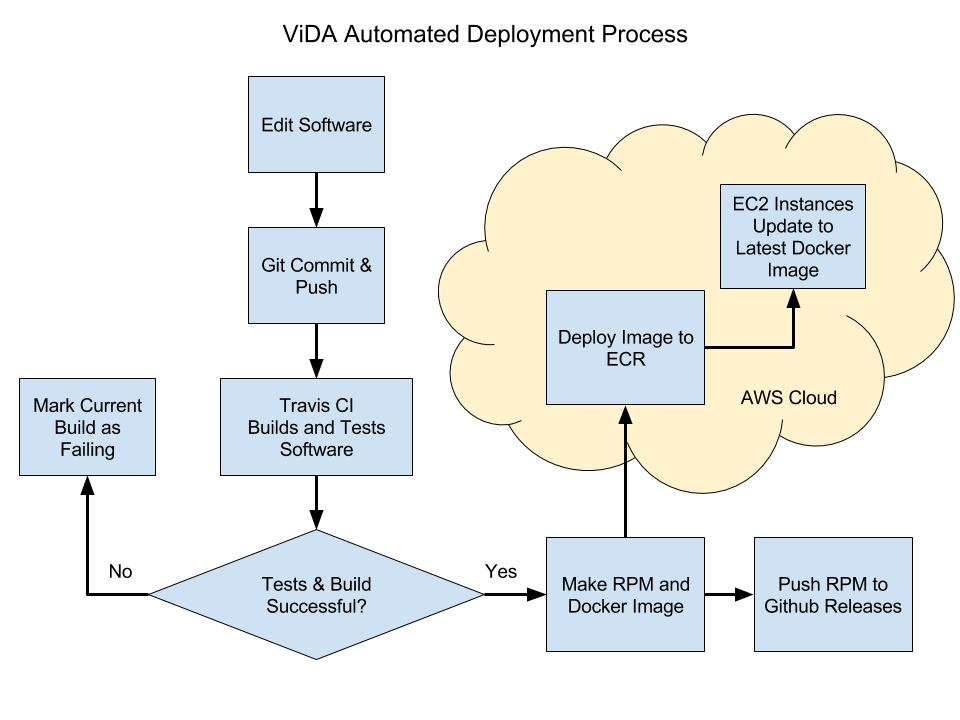
\includegraphics[width=\textwidth]{figures/continuous_integration}
  \caption{Automated deployment of the proposed feature extraction method to
  the AWS cloud using continuous integration}
  \label{fig:continuous_integration}
\end{figure}

\subsection{\label{subsection:tdd}Test Driven Development}
For the majority of our C++ development, we used a software engineering technique
called test driven development (TDD) \cite{beck2003test}. This technique is germane to
our method's section because repeatability of our experiments and future
extension of our work depends on well developed, robust software. The main idea is that
before we ever wrote code to implement a new algorithm, we first design a failing
test and then write code to make that test pass. This has several advantages over
not writing tests for code:

\begin{itemize}
\item It gives developers a predictable way to code. Rather than thinking
abstractly about what goals a developer is attempting to accomplish, the developer
writes concrete tests that should validate the behavior that is desired.
\item It allows for lessons to be learned early on about the implementation details
of the software. If a developer delves directly into solving a software problem
with a single mindset about how it should be implemented, then the opportunity
for a different design pattern to be used is extinguished. The main idea being
that if test driven development is used for designing an algorithm then the best
design pattern for the problem will be chosen, not just the one the developer
is familiar with.
\item Test driven development forces developers to be accountable. All too often
code is written with the mindset that its okay to commit hundreds or even
thousands of lines of code most of which is barely tested. And thus the code
becomes riddled with bugs and other developers end up having to fix those issues.
With TDD, this is a less frequent occurrence because developers must write a test
for every logical unit of code.
\end{itemize}

For this thesis we use TDD to develop our extract features program and to design
several programs that we use for experimental purposes. In order to facilitate
the development, we use google test as our C++ testing framework
\cite{googletest}. An example of a test we have written to test receiving a
single video frame from a file is shown in Appendix \ref{ap:google_test}. This
test uses a concept from the TDD community known as a mocked object. The
philosophy behind using a mocked video reader as illustrated in the test, is
that we don't want to design our tests to be reliant on the state of the current
system. If we do so, the second we push our code to the repository, our
continuous integration tool will fail. Mocked objects give us the ability to
test our algorithms without having to rely on the state of our development
machine, the network or other variable elements. This is a powerful concept
because it ensures that our tests run fast and also forces us to program to
interfaces rather than concrete objects. In order to fully leverage the power of
mocked objects, we use a design pattern, as shown Appendix \ref{ap:google_test},
known has dependency injection \cite{gamma1995design}. The idea behind
dependency injection is that we can inject our dependencies into an algorithm at
runtime or compile time to have our object get the resources it needs to perform
a calculation in a variety of ways. For example, in our test in Appendix
\ref{ap:google_test}, we inject the interface called ``Reader''. ``Reader'' is a
specific example of high-performance dependency injection because no virtual
interfaces are used. This concept can only be used at compile time and the
interfaces cannot be swapped out at runtime. High performance dependency
injection is achieved by using only templates, which by their nature, can only
be determined at compile time and not run time. In order to achieve type
inference at runtime, we would need to use a virtual interface instead which has
the additional overhead of doing a virtual table lookup. As a result of using
this reader interface instead of using OpenCV's video reading capabilities, we
give ourselves the flexibility to read from hierarchical data format (HDF5)
files, a web interface, or anything as long as we adhere to the contract we have
defined in the interface code. And thus we can also write a mocked object, which
is to say, an object that we can easily define the inputs and outputs of on the
fly so that we can test a variety of scenarios in our motion estimation
algorithm without having to rely on any external resources. Figure
\ref{fig:hiperf_dependency} illustrates how dependency injection looks for our
MotionEstimation class.

\begin{figure}[h]

  \centering
  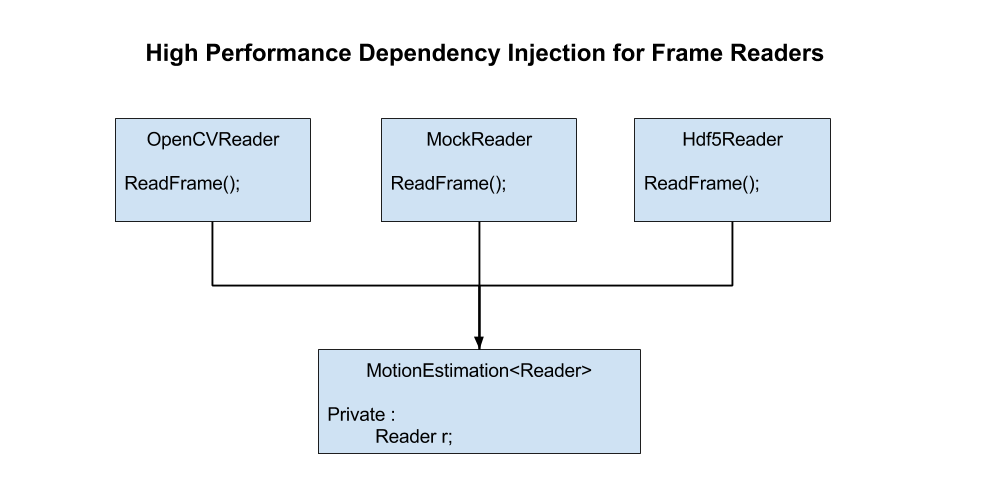
\includegraphics[width=\textwidth]{figures/dependency_injection}
  \caption{High performance dependency injection using templates to implement the
  motion estimation class with different types of video readers.}
  \label{fig:hiperf_dependency}
\end{figure}

The appendix example demonstrates how we now have a failing test, and we can then
begin implementing the code that causes test to pass. As a result, if we
push our failing test to Github, our current build will not be deployed to the cluster
until we have our tests passing. Figure \ref{fig:passing} illustrates what a commit
looks like when it is passing on our Github project and Figure \ref{fig:passing}
shows what it looks like when the build is failing because of a test, compilation
issues, or problems pushing to the AWS cloud.

\begin{figure}[h]

  \centering
  
\includegraphics[width=\textwidth]{figures/passing}
  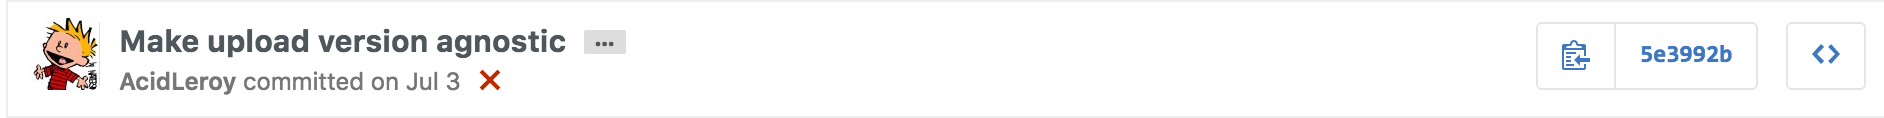
\includegraphics[width=\textwidth]{figures/failing}
  \caption{An example of two commits that were pushed to our repository. The
  top figure shows how the build is marked as passing with a green check mark,
  and the bottom shows the build failing with a red x.}
  \label{fig:passing}
\end{figure}


\section{\label{section:vida_oflow} Implementing Optical Flow }
In our software, we use two OpenCV library calls, \texttt{goodFeaturesToTrack}
and \\
\texttt{calcOpticalFlowPyrLK} to implement the Lucase-Kanade Pyrmidal optical
flow. The first function is used to find features that can be easily tracked
from one frame to the other using the Shi-Tomasi algorithm \cite{shi1994good}.
The next method then calculates the optical flow between the good points using
the pyramidal implementation of the Lucas-Kanade algorithm
\cite{bouguet2001pyramidal}. Figure \ref{alg:lk_flow} outlines the general
program flow for calculating motion vectors in the proposed feature extraction method.

\begin{figure}[h]
\begin{algorithmic}[1]
\Procedure{CalculateVectors}{$frame1$, $frame2$}
  \If{\text{$track\_points\_initialized$}}
  	\State $opticalflow \gets \texttt{calcOpticalFlowPyrLK}(track\_points, frame1, frame2)$
  \Else
  	\State $track\_points \gets \texttt{goodFeaturesToTrack}(frame1)$
	  \State $track\_points\_initialized \gets True$
	  \State $optical\_flow \gets  \texttt{CalculateVectors}(frame1, frame2)$
  \EndIf
  \Return $optical\_flow$
\EndProcedure
\end{algorithmic}
\caption{Calculating Lucas-Optical Flow from Videos}
\label{alg:lk_flow}
\end{figure}

The algorithm used in our proposed architecture is similar to Figure \ref{alg:lk_flow} but
contains fewer steps since there is no need to get good features to track.
In the C++ software, we also implemented Farneback method. The
Farneback implementation is shown in Figure \ref{alg:farneback}.

\begin{figure}[h]
\begin{algorithmic}[1]
\Procedure{CalculateVectors}{$frame1$, $frame2$}
  \State $optical\_flow \gets \texttt{calcOpticalFlowFarneback}(frame1, frame2)$\\
  \Return $optical\_flow$
\EndProcedure
\end{algorithmic}
\caption{Calculating Farneback Flow from Videos}
\label{alg:farneback}
\end{figure}

As can be seen in \ref{alg:farneback}, we don't need any good features to track
because we are calculating the optical flow globally between frames, rather than
selecting a few features. This has the advantage of tracking optical flow objects
that may fail the Shi-Tomasi method for tracking, but because it is no discriminant
in the features, the resulting motion vectors are dense.


\section{\label{section:comparison}Comparison of Methods}
We implemented the Lucas-Kanade method first in our research because in general,
performance is a concern and, as long as not too many features or
too few features are detected, the Lucas-Kanade algorithm will be faster
\cite{de2015choosing}. Despite this fact, we found that our classifier did
not perform as well on features extracted from the Lucas-Kanade method, as it
did using the Farneback method. Hence most of the results in this thesis
have been calculated with Farneback optical flow unless otherwise specified.

\section{\label{section:feature_extraction}Feature Extraction from Optical Flow}
The first step that needs to be done in our software is to open a video file.
All of the videos that are used in this thesis are compressed before reaching an
S3 bucket, and then are later decompressed  within each compute node. This is
important to note because bandwidth is a limiting factor when transferring
videos from an S3 bucket to the compute node.  Therefore the first step is to
have OpenCV read the file in and decompress it before  reducing the feature
space. Figure \ref{fig:life_of_video} illustrates how a video is first read in
to extracting the features from each of the cropped videos producced. The
\texttt{CalculateVectors} function in both Figure \ref{alg:lk_flow} and
\ref{alg:farneback} returns several dense matrices that represent the features
that we can extract from the optical flow output. These features are magnitude,
orientation, x direction and y direction of the optical flow features. These are
ultimately the features that we use to train and classify using an SVM. However,
if we had two $N \times M$ video frames as the input, we now have $4 \times N
\times M$ features. Clearly we have not yet reduced the input feature space.
Thus, based on information that we know \textit{a-priori}, we can reduce our
feature space significantly.

\begin{figure}[h]
  \centering
  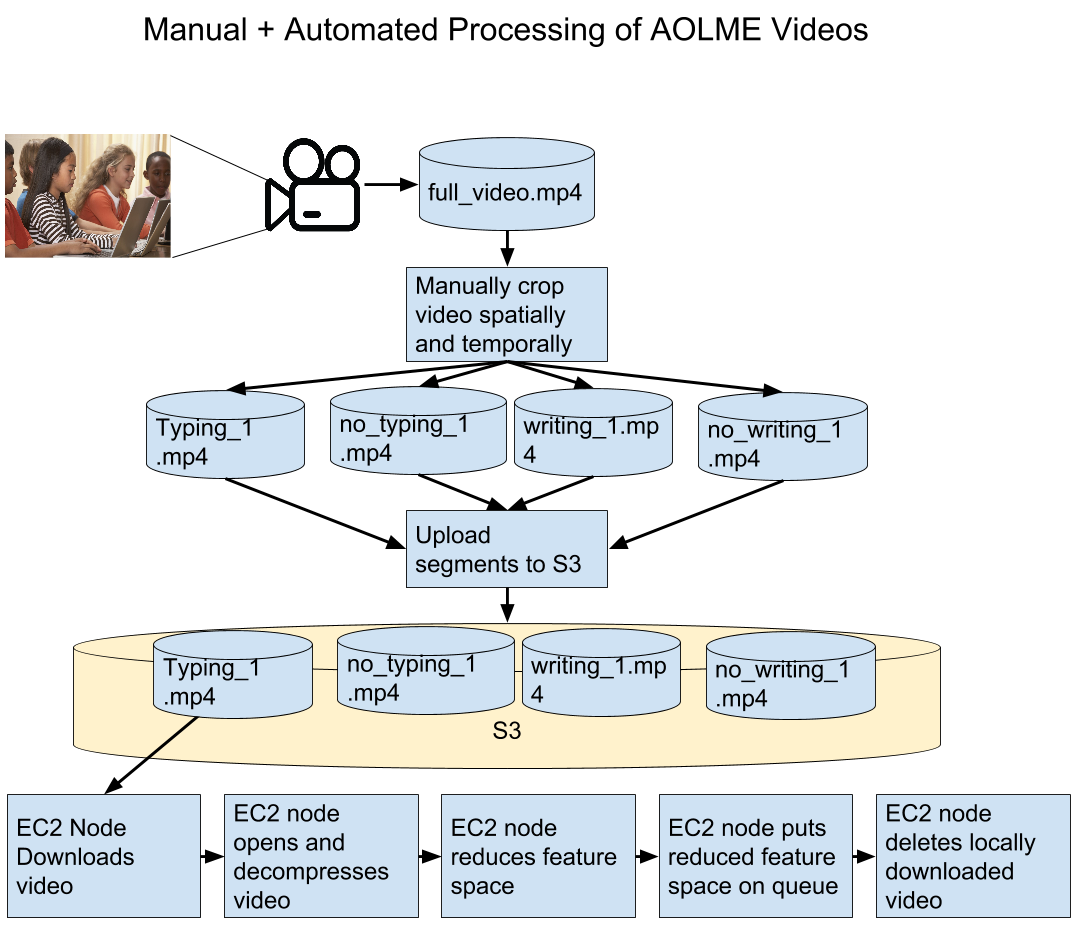
\includegraphics[width=\textwidth]{figures/life_of_video}
  \caption{Processing of a single raw video to feature extraction as implemented
  in the proposed architecture.}
  \label{fig:life_of_video}
\end{figure}

\FloatBarrier

In the case of typing and writing, we know we can expect there to be motion from
one frame to the next. We don't know by how much, but we do know that it is not
zero. Using this knowledge, we can then threshold the optical flow vectors that
we get back from Figure \ref{alg:lk_flow} and \ref{alg:farneback}. The
threshold value used was empirically calculated from doing multiple runs on the
AOLME videos. We found we got the best results by only retrieving
optical flow vectors with a magnitude greater than 75\% of the max value. The set
of Equations in \ref{eq:optical_threshold} illustrate this idea.

\begin{align}
  \begin{split}
  \mathbf{V} &= (\mathbf{V_x}, \mathbf{V_y}) \\
  \mathbf{V_m} &=
  \begin{cases}
    1, & \text{if } \|\mathbf{V}\| \geq \max( \|\mathbf{V}\|) \times 0.25 \\
    0, & \text{otherwise}
  \end{cases}
  \end{split}
  \label{eq:optical_threshold}
\end{align}

where $\mathbf{V_x}$ and $\mathbf{V_y}$ are the optical flow vectors in the
x and y directions respectively. $\mathbf{V_m}$ is the bit mask that is
then used to extract the subset of data from each of the dense matrices.

\begin{align}
  \begin{split}
  \text{Let: } \\
  \|\mathbf{V\prime}\| &= \|\mathbf{V}\| \circ \mathbf{V_m}\\
  \mathbf{V_x\prime} &= \mathbf{V_x} \circ \mathbf{V_m}\\
  \mathbf{V_y\prime} &= \mathbf{V_y} \circ \mathbf{V_m}\\
  \mathbf{\Phi\prime} &= \mathbf{\Phi} \circ \mathbf{V_m}
\end{split}
\label{eq:subset}
\end{align}

Using the optical flow bitmask, $\mathbf{V_m}$, we can then extract features
from each one of our dense matrices using the Hadamard product as shown in
Equation \ref{eq:subset}, where $\|\mathbf{V\prime}\|,
\mathbf{V_x\prime},\mathbf{V_y\prime}, \mathbf{\Phi\prime}$ are subset matrices
for the magnitude, x and y direction and orientation respectively. We have now
reduced the feature space somewhat, but depending on the size of the video and the
amount of entropy per frame pair, we could still have a significant amount of
data to process for classification, this idea is especially true for
Farneback optical flow.

In addition to extracting generic vectors from the video, we also add
geometrical centroids, blob orientation and background motion around the blobs
to the optical flow statistics being used for classification. We implement these
methods to attempt to leverage information that could be useful during
classification. In order to calculate the geometrical centroids and orientations
of each blob, we use some well known algorithms available in OpenCV,
\texttt{connectedComponentsWithStats} and \texttt{findContours}
\cite{itseez2015opencv}. \texttt{connectedComponentsWithStats} is a function
that allows us to compute the centroid for each blob of connected pixels. The
input to this function is our binary mask image, $\mathbf{V_m}$. Once we have
all the connected blobs, we can then calculate the orientation of each one of
those blobs using \texttt{findContours} in combination with with
\texttt{fitEllipse}. The full implementation of this algorithm is outlined in
Appendix \ref{ap:centroids}. The final step is to then dilate each blob, and
then retrieve the magnitude of the optical flow in this region. Appendix
\ref{ap:dilate} gives the C++ code that was used for these calculations.
Figure \ref{fig:orient_cent} illustrates the idea of acquiring
the centroid and orientation of the blobs from $\mathbf{V_m}$.

\begin{figure}[h]
  \centering
  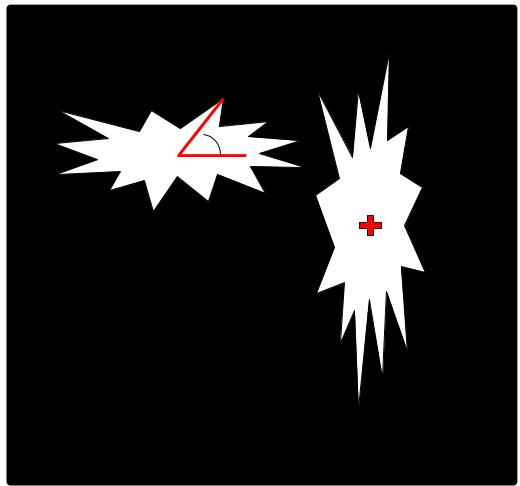
\includegraphics[width=8cm]{figures/cent_and_orient}
  \caption{Example of orientation measurement on the left, and the centroid
  calculation on the right.}
  \label{fig:orient_cent}
\end{figure}

When the previous optical flow features have been generated, their values are
then organized into a probability density function (PDF) with 25 bins. That is
to say that each frame pair generates a PDF and that PDF is accumulated for
every subsequent frame in the video sequence. When our software reaches the end
of the video file, a normalized, cumulative distribution function (CDF) is
calculated and output for each vector. So for each input video there will be one
CDF with 25 bins for blob orientation, blob centroid x and y, motion vector
magnitude, motion vector orientation and background motion vector magnitude.
Figure \ref{fig:extract_flow} clearly illustrates this concept.

\begin{figure}[h]
  \centering
  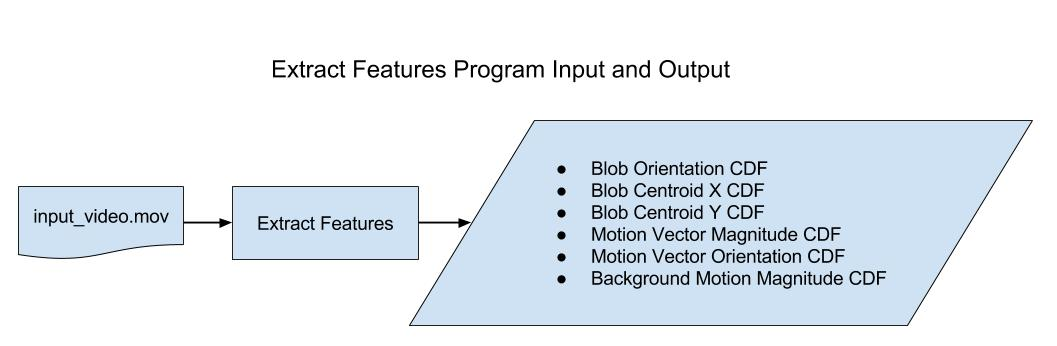
\includegraphics[width=\textwidth]{figures/extract_features_flow}
  \caption{Flow of the extract features program. For every input video, it will
  return a CDF with 25 bins for each of the extracted features from the motion
  vectors}
  \label{fig:extract_flow}
\end{figure}

Ultimately, these are the features that are then accumulated for multiple AOLME
videos and used for classification.

\section{\label{section:classification}Classifying the Reduced Feature Space}
At this point we now have accumulated a bag of features for videos. The features
that are collected are stored in a comma separated file (csv) that can be read
in by the any of the popular machine learning packages such as those provided
by the R language or Python's SciKit-Learn. The file contains labels that have
filename, centroid x CDF, centroid Y CDF, background motion CDF, motion magnitude
CDF, motion orientation CDF and classification. We can then use an SVM to classify
the features. To validate our results, we use leave-one-out cross validation
to ensure that we have not overfit the data.

This thesis uses the SVM software that is included in the R language for
accurate classification. The algorithm is based off the original paper written
by Vapnik \cite{cortes1995support} but was then much improved for computational
efficiency by Chang \& Lin in 2011 \cite{chang2011libsvm} with their award
winning software package known as LIBSVM. This library was originally written
in C, but many fans of the algorithm have created software bindings for multiple
languages, including R.

The classification of our feature vectors is very simple since the majority of
the hard work has already been implemented in the machine learning algorithms
we use to do the classification. The process is as follows


\begin{itemize}
  \item Load features from CSV file into an R data frame
  \item Plot statistics about the features
  \item Loop over data frame using leave one out cross correlation
  \item Select most accurate results between K nearest neighbors and tuned, non-linear
  support vector machine.
\end{itemize}

The R code used to do the classification is shown in Appendix
\ref{ap:svm_classification}.
